\subsection*{Introduzione teorica}

Si vuole studiare il problema agli autovalori:
$$ \Hh\psi = E \psi $$
%
Siano $k^2 = 2E$ e  $q^2 = 2(E-V0)$. La soluzione analitica più generale è data da:
%
$$
\psi_k(x) =
    \begin{cases}
        Ae^{ikx}+Be^{-ikx} & \mbox{in ZonaI} \\
        \phi(x) & \mbox{in ZonaII} \\
        Ce^{ikx}+De^{-ikx} & \mbox{in ZonaIII} \\
    \end{cases}
$$
%
\bigskip
Non siamo per il momento interessati alla ZonaII, quindi indichiamo con
$\phi(x)$ la $\psi_k(x)$ in tale zona, che a rigore sarebbe
    $$\phi(x)= Ee^{iqx}+Fe^{-iqx}$$
Le costanti $A,B,C,D$ sono determinate dalle condizioni di raccordo di continuità della
funzione d'onda e della sua derivata nei punti $x=\pm b$.\\
Si osserverà che dalla diagonalizzazione della versione discreta della Hamiltoniana
(vedi sezione apposita) risultano autofunzioni a parità definita (pari o dispari).
Allora, senza perdita di generalità, si pone la ulteriore condizione di simmetria alle $\psi_k$, che porta:
$$\begin{cases}
    A = D, \qquad  B = C = (\tau + \rho)A &\mbox{per funzioni pari} \\
    A = -D, \quad B = -C = -(\tau + \rho)A &\mbox{per funzioni dispari}\\
\end{cases}$$
Per la conservazione del flusso di probabilità, si possono riscrivere nella seguente forma:
$$
    \begin{pmatrix} C \\ B \end{pmatrix} =
    \begin{pmatrix} \tau & \rho \\ \rho & \tau \end{pmatrix} \cdot
    \begin{pmatrix} A \\ D \end{pmatrix} = \quad (S)\cdot \begin{pmatrix} A \\ D \end{pmatrix}
$$
Ove la matrice S è una matrice unitaria, che di conseguenza verifica le condizioni:
$$ \tau\rho^* + \tau^*\rho = 0 \quad,\quad |\tau|^2 + |\rho|^2 = 1$$
(Si è indicato con $z^*$ il numero complesso coniugato di $z$). Segue immediatamente che:
$$ |\tau \pm \rho|^2 = |\tau|^2 + |\rho|^2 + \tau\rho^* + \tau^*\rho = |\tau|^2 + |\rho|^2 + 0 = 1$$
Cioè $\tau \pm \rho$ differiscono per una fase:
$$ |\tau \pm \rho|^2 = 1 \Rightarrow (\tau \pm \rho) = e^{2i\theta^\pm}$$
Si osservi che poichè $A,B,C,D$ dipendono dagli autostati $\psi_k$, anche le fasi $\theta^\pm$ dipenderanno dall'autovalore $k$.\\
Si vuole quindi cercare una stima numerica di $\theta\pm$ per determinare $\tau$ da:
    $$ (\tau \pm \rho) = e^{2i\theta^\pm} \Rightarrow \tau = 1/2(e^{2i\theta^+}+e^{-2i\theta^-})$$
    $$ \Rightarrow \tau^2 = \sin^2(\theta^+ - \theta^-)$$
(due conti per dimostrarlo plis) (OCCHIO che esce un coseno)
\\
Il coefficiente di trasmissione sarà qundi dato da:
    $$T = \tau^2$$

\subsection*{Stima delle Fasi}
Si vuole stimare numericamente le fasi $\theta^\pm$, a partire dagli autovettori
calcolati dalla $\Hh$ discretizzata. Gli autovettori sono combinazioni pari e dispari
di onde piane con la stessa frequenza, quindi corrispondono rispettivamente a coseni e seni.
    $$ \psi_k^{odd} = \begin{cases}
        A\sin(kx + \theta^-_k) & \mbox{in ZonaI} \\
        A\sin(kx + \theta^+_k) & \mbox{in ZonaIII} \\
    \end{cases}
    \quad
    \psi_k^{even} = \begin{cases}
        A\cos(kx + \theta^-_k) & \mbox{in ZonaI} \\
        A\cos(kx + \theta^+_k) & \mbox{in ZonaIII} \\
    \end{cases}
    $$

\begin{paragraph}{Primo Metodo}
Si vuole fittare i dati con seni e coseni di opportuna frequenza $k$
e fase da determinare (parametro di fit). Si definiscono allora:\\
  In ZonaI = $\{x<-b\}$, sia
        $$f^{even}_k(y) = \int_{-\infty}^{-b} | A\cos(kx+y)-\psi_k^{even}(x)| \mathrm d x $$
        $$f^{odd}_k(y) = \int_{-\infty}^{-b} | A\sin(kx+y)-\psi_k^{odd}(x)| \mathrm d x $$
  In ZonaIII = $\{x<-b\}$, sia
        $$g^{even}_k(y) = \int_{b}^{+\infty} |A\cos(kx+y)-\psi_k^{even}(x)| \mathrm d x $$
        $$g^{odd}_k(y) = \int_{b}^{+\infty} |A\sin(kx+y)-\psi_k^{odd}(x)| \mathrm d x $$
Si ha immediatamente che:
    $$ \theta^-_k = y \mbox{ t.c. } f_k(\theta^-_k) = 0 $$
    $$ \theta^+_k = y \mbox{ t.c. } g_k(\theta^+_k) = 0 $$
\end{paragraph}
Si troverà che:
    $$ \theta^+_k = -\theta^-_k = \theta_k $$
Quindi:
$$ \psi_k^{odd} = \begin{cases}
    A\sin(kx - \theta_k) & \mbox{in ZonaI} \\
    A\sin(kx + \theta_k) & \mbox{in ZonaIII} \\
\end{cases}
\quad
\psi_k^{even} = \begin{cases}
    A\cos(kx - \theta_k) & \mbox{in ZonaI} \\
    A\cos(kx + \theta_k) & \mbox{in ZonaIII} \\
\end{cases}
$$

\begin{paragraph}{Secondo Metodo}
Si considerino i punti $x = \pm 2\pi$, siano $y(\pm 2\pi)$ i valori degli autovettori
numerici in quei punti, separatamente pari e dispari. Si ha allora che:
$$ \begin{cases}
    y^{odd}(2\pi)   = \sin(k2\pi  + \theta_o^+)  & \Rightarrow \theta_o^+ = \arcsin(y^{odd}(2\pi)) - k2\pi\\
    y^{odd}(-2\pi)  = \sin(-k2\pi + \theta_o^-)  & \Rightarrow \theta_o^- = \arcsin(y^{odd}(-2\pi)) + k2\pi\\
    y^{even}(2\pi)  = \cos(k2\pi  + \theta_e^+)  & \Rightarrow \theta_e^+ = \arccos(y^{even}(2\pi)) - k2\pi\\
    y^{even}(-2\pi) = \cos(-k2\pi + \theta_e^-)  & \Rightarrow \theta_e^- = \arccos(y^{even}(-2\pi)) + k2\pi\\
\end{cases}$$
\end{paragraph}
Di seguito il plot del risultato\\
%% Sarebbe bello che stesse sulla stessa pagina
\begin{figure}[h]
  \centering
  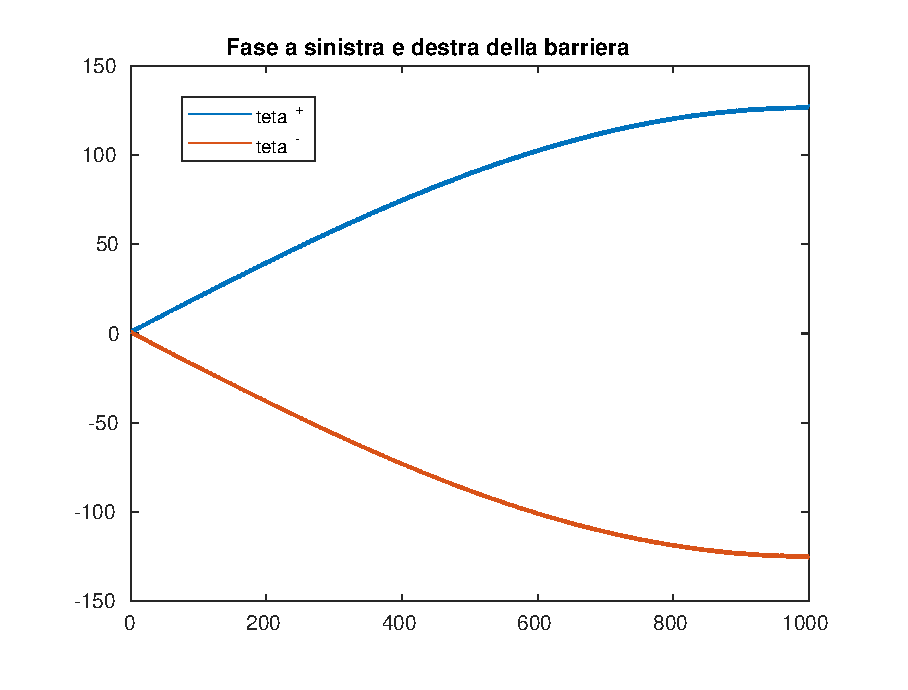
\includegraphics{fasi.eps}
\end{figure}
%
\newpage
\subsection*{Risultati}
Di seguito il plot del coefficiente di trasmissione calcolato numericamente contro
il risultato analitico

%% Immagine da mettere sotto la frase, possibilmente in una unica pagina
\begin{figure}[h]
  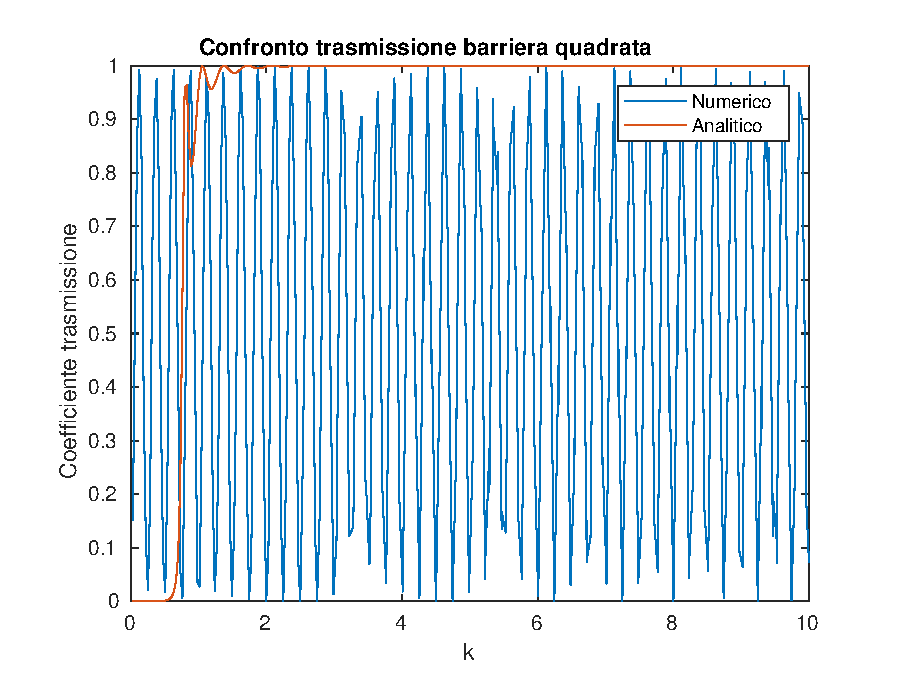
\includegraphics{tr_coeff_square.eps}
\end{figure}
